\documentclass[10pt,twocolumn]{article}

% use the oxycomps style file
\usepackage{oxycomps}

% usage: \fixme[comments describing issue]{text to be fixed}
% define \fixme as not doing anything special
\newcommand{\fixme}[2][]{#2}
% overwrite it so it shows up as red
\renewcommand{\fixme}[2][]{\textcolor{red}{#2}}
% overwrite it again so related text shows as footnotes
%\renewcommand{\fixme}[2][]{\textcolor{red}{#2\footnote{#1}}}

% read references.bib for the bibtex data
\bibliography{references}

% include metadata in the generated pdf file
\pdfinfo{
    /Title (Experimenting with Strategies to Overcome Insufficient Training Data for Spanish - Nahuatl Translation)
    /Author (Ryann Hally)
}

% set the title and author information
\title{Experimenting with Strategies to Overcome Insufficient Training Data for Spanish - Nahuatl Translation}
\author{Ryann Hally}
\affiliation{Occidental College}
\email{hally@oxy.edu}

\begin{document}

\maketitle

\section{Introduction}
For my comprehensive requirement, I trained Google's T5 Transformer model to translate Spanish text into Nahuatl, an indigenous language spoken in present day Mexico. I experimented with strategies to make up for the small amount of training data in this language pair, and analyzed how each strategy affected model performance.

\section{Problem Context}

Translation systems that use machine learning (ML) far outperform rule-based approaches, producing translations that are both more fluent and more accurate. However, they must be trained on massive amounts of data. Google estimates that for a ML-based translation system to correctly translate a language of the morphological type that Nahuatl is, it would need roughly 5 million parallel examples  \cite{Chen}. The largest publicly available corpus for Spanish-Nahuatl is consists of roughly 20,000 example translations, which comprises around .4\% of the necessary training data \cite{SomosNLP}. Unsurprisingly, current Spanish-Nahuatl ML-based translation are not able to produce many accurate translations. Thus, I decided to experiment with strategies to improve translation accuracy for Spanish-Nahuatl ML-based translation.

There are many reasons why creating an accurate automatic Spanish-Nahuatl translator is important. First, there are almost 2 million Nahuatl speakers, and 15\% of these speakers are considered monolingual \cite{Nahuatl}. Automatic translators are helpful tools for looking up words or translating online resources like websites, which would be particularly useful for monolingual Nahuatl speakers. Second, although Nahuatl is one of the most widely spoken indigenous languages in central America, it is experiencing a decline in  number of speakers \cite{Nahuatl}. Creating a working translator will enable resources such as government websites or even books to be automatically translated into Nahuatl, allowing speakers to the use language more in their daily life and thus reviving it it \cite{SomosNLP}. More broadly, the vast majority of the world's indigenous languages are experiencing declines in speaker population \cite{IndigenousLanguageDeath}. Due to the small amount of speakers they have, there isn't enough data in them to train a translation system. In other words, the languages that could benefit most from automatic translation are the same languages in which there isn't enough resources to make a translator.  Thus, it's important we learn to create usable and accurate translators with small amounts of data. 


This project was difficult to execute. The technologies I worked with were difficult to understand conceptually (transformer architecture, word embeddings, attention mechanisms, etc). Additionally, I taught every step of the machine learning pipeline: data processing, tokenization, training, and evaluation. 


\section{Technical Background}
Next, I will describe the concepts necessary to understand the project. 

\subsection{Linguistic Terminology}

\subsubsection{Morpheme}

A morpheme is a the smallest unit of language that has independent meaning. In English, "general" and 'ly" are the morphemes that form the word "generally". \cite{Polysynethic}


\subsubsection{Morphology}

A language's morphology is the way morphemes come together to form words in the language.  \cite{Polysynethic}


\subsubsection{Polysynthetic}

In polysynthetic languages, several morphemes can be added together in order to form long, complex words that might constitute entire sentences in English. \cite{Polysynethic}
For example, the Nahuatl word \textit{ichipilli} can be translated to English as "I am a poor humble women." 


\subsection{Machine Learning and Translation Terminology}
\subsubsection{Low-resource Languages and Language Pairs}

If there isn't enough data in a language pair (translating from one particular language into another) to create an ML-based translator, it is considered a low-resource language pair. Chen (2022) \cite{Chen} defines a low-resource language pair as any language pair in which there are less than .5 million parallel translation examples. Languages on their own can be considered low-resource if there generally isn't enough data to translate into or from them from any language. The language Nahuatl as well as Spanish-Nahuatl the language pair are both considered low resource \cite{Chen} \cite{SomosNLP} .

\subsubsection{Parallel Corpus}

The dataset I used to train T5 is a parallel corpus. A parallel corpus feature words, phrases, or paragraphs in one language with corresponding translations in one or more languages. Translations are aligned at either the word or sentence level. The parallel corpus I use features Spanish words and phrases with their corresponding Nahuatl translations. 


\subsection{Architecture and Model}

In machine learning, a model is a trained machine learning algorithm. On the other hand, an architecture is a  set of components that make up a machine learning model. \cite{Architecture}


\subsection{Transformers}

Transformers are a type of machine learning architecture. They are characterized by their use of feed forward neural networks and attention mechanisms. Transformers capture dependencies between words through attention mechanisms, which weight parts of a sequence for how relevant they are to the the particular word or subword being translated and allow the transformer to focus on the most relevant parts. \cite{Transformers}


\subsection{Tokenizer}

Tokenization is the main step in preprocessing the training data. Data cannot be fed to the model as text, and it must instead be represented numerically. Tokenizers break down text into words, subwords, or characters, and convert them into numerical representations called tokens \cite{Tokenizers}.  


\subsection{Epochs and Training Duration}

An epoch is one pass through the entire dataset during training. Training duration is generally measured is number of epochs, as it provides a more consistent measure than time elapsed, which can vary significantly based on device used and dataset size. \cite{Epoch}

\subsection{Cross-lingual Transfer Learning}
The underlying concept of transfer learning is to apply knowledge from one task to a different but related task. In machine translation, cross-lingual transfer learning refers to first training a model in translation between one language pair before training it in translation between another language pair. For example, a model could be trained in English-Spanish before English-French. \cite{Ren}

\subsection{Orthography Normalization}
A language's orthography refers to the conventions around how it is written. Orthography normalization involves standardizing or making consistent an orthography. \cite{Elotl}


\section{Prior Work}

I will start by discussing prior work around ML-based translating systems for low resource indigenous languages, and then highlight a few projects that focused on Spanish-Nahuatl translation.

\subsection{Machine Translation for Low Resource Indigenous Languages}

Ngoc Le (2020) \cite{NgocLe} , Ren (2021) \cite{Ren},  Zheng (2021) \cite{Zheng} and Chen (2022) \cite {Chen} use machine learning to create translation systems for low-resource indigenous languages.

Ngoc Le (2020) \cite{NgocLe} experiments with translation into Inuktitut, a indigenous language of Canada while Ren (2021) \cite{Ren}, Zheng (2021) \cite{Zheng} and Chen (2022) \cite {Chen}  all focus on South America indigenous languages. Ren (2021) \cite{Ren} narrows in on Spanish-Quechua translation while Zheng (2021) and Chen (2022) translate Spanish into 10 different South American languages. While the corpus sizes used in each experiment varies, since the four studies are investigating translation for low resource languages they all contain less than 500,000 pairs.

In terms of the models used, Zheng (2021) \cite{Zheng} and Chen (2022) \cite {Chen} employ mBart while Ren (2021) \cite{Ren} uses openNMT. Ngoc Le (2020) \cite{NgocLe} does not disclose the exact model used but describes it as adjacent to BERT. Thus, all four studies use neural machine translation (NMT) transformer models.

All four studies use automatic evaluations metrics to asses translations. Ngoc Le (2020) \cite{NgocLe} uses BLEU on its own, whereas Chen (2022) \cite {Chen} , Zheng (2021) \cite{Zheng}, and Ren \cite{REN} employ both BLEU along with chrF. I choose to use both BLEU, or rather a variant of BLEU called sacreBLEU, and chrf  in my own project, both to assess the translations my models produced and to compare my results with their work. 

Zheng (2021) \cite{Zheng}, Chen (2021) \cite {Chen}  and Ren (2021) \cite{Ren} all experiment with cross-lingual transfer learning. Ren (2021) \cite{Ren} uses a pretrained Spanish-Finnish model for Spanish-Quechua, selecting Spanish-Finnish because of Finnish's morphological similarity to Spanish. They report an improvement of +9.852 BLEU and +0.177 chrF with the Spanish-Finish pretrained model, clearly demonstrating the effectiveness of pretraining. Chen (2022) \cite {Chen} uses bilinugal models pretraineed in Spanish-Catalan, Spanish-English, and Spanish-Romanian as well as multilingual models pretrained in over 20 languages. They find that the multilingual models achieve higher BLEU and chrF scores for all 10 of the indigenous languages they experiment with. Interestingly, Zheng (2021) \cite{Zheng} uses monolingual data instead of a language pair for translating. However, the purpose of their study is not to identify the effectiveness of pretraining and they therefore do not create a non pretrained model to compare their results too.

Chen (2022) \cite {Chen} sees improvement through using multilingual models and Ren (2021) \cite{Ren} notes considerable increases in BLEU with pretraining. However, none of the studies come close to creating a translation system where the majority of translations are accurate as judged by to BLEU and chrF. For example, none of the fours studies report a chrF  score higher than 1/100. Their work highlights the difficulty of the creating a translator with so little data but the possibility for improvement through experimentation. 


\subsection{Spanish-Nahuatl Translation}

I will now discuss prior work on ML-based translation for Spanish-Nahuatl. Zheng (2021) \cite{Zheng} and Chen (2022) \cite {Chen}  both include Nahuatl as on one of the indigenous languages they experiment with, translating into the language from Spanish. The other project I looked to was the winner of the SomosNLP organziation's Spanish-Nahuatl translation hackathon \cite{SomosNLP}.

Like Zheng (2021) \cite{Zheng} and Chen (2022) \cite {Chen}, SomosNLP \cite{SomosNLP} uses a transformer NMT model. They employ Google's T5, which led me to discover and select it as the model for my project.

SomosNLP \cite{SomosNLP} employs a unique technique for overcoming insufficient data . They add 20,000 pairs (the same size as the Spanish-Nahuatl corpus they use) of English-Spanish data to their training data. The English-Spanish data is included in the training corpus as if it were Spanish-Nahautl data. This is not an example of pretraining, since pretraining is done beforehand and as a seperate process from training in the low-resource language.

Like Zheng (2021) \cite{Zheng} and Chen (2022) \cite{Chen}, the SomosNLP \cite{SomosNLP} winners use cross-lingual transfer learning to improve model performance. They pretrain in Spanish-English with 100,000 pairs and report small increases in both sacreBLEU and chrF. 

SomosNLP \cite {SomosNLP }reports a sacreBLEU score of 6.18 and a chrF score of 28.21 for Spanish-Nahautl translation, while Zheng (2021) \cite{Zheng} and Chen (2022) \cite{Chen} report BLEU scores of 1.2 and 2.947 and chrf scores of 0.238 and 0.3015. 

\section{Methods}
Next, I will explain the methods I used to complete my project and why I choose them. 

\subsection{Google T5-Small}
I chose to train Google's T5-Small transformer model for a number of reasons.

First, T5 is a transformer NMT model. All the prior work I read into translation for low-resource indigenous languages utilized this type of model. Additionally, my research into the available approaches, architectures, and models for translation indicated that NMT transformers produced the most accurate and fluent translations \cite{Transformers}. This is due in large part to their use of  attention mechanisms as discussed previously. 

Secondly, T5's text-to-text prefix strategy allows for easy pretraining. When training T5 on a new task, a prefix is added to the input data \cite{T5Model}. For example, I attached the prefix "Translate Spanish to Nahuatl: " to each of the Spanish words and phrases I fed the model. The same model can therefore be trained for new tasks, and the process is simple and seamless.

Third, T5 comes pretrained in 4 different languages.  T5 is pretrained in English, French, German, and Romanian \cite{T5Model}. Since my Spanish-Nahautl dataset was so small, I looked for a model that was already trained for NPL tasks in other languages to help make up for the lack of data.


\subsection{Tokenizer}
I used T5's accompanying sentence piece tokenizer. I considered using a different tokenizer, such as one geared towards segmenting polysynthetic languages like Nahuatl. However, I decided to stick with T5's tokenizer to be certain it was compatible with the T5 model. 

\subsection{Corpus}
I used SomosNLP's Spanish-Nahuatl dataset, which consists of 12,000 Spanish-Nahuatl pairs taken from two smaller datasets. Roughly 12,000 pairs come from the Axolotl corpus \cite{AxolotlCorpus} \, , which is made up of a mixture of recipe books, poems, and historical documents that have been translated from Spanish into Nahautl or vice versa. The 12,000 pairs do not constitute the entire corpus, but a subset that are considered well-aligned \cite{SomosNLPDataset} .  The remaining 8,000 pairs come from Bible-UED corpus, which is a corpus of bible translations. The orthography is normalized using Py-elot's "sep" normalizer.

\subsection{Training and Test Sets}
I split each dataset into a training and test (commonly called validation) set. I put 90\% of each dataset into the training set and set aside 10\% for validation. This was based on SomosNLP's  work \cite{somosNLP} .

\subsection{Training Hyperparameters}
I trained each model for 280 epochs, except for when I was experimenting with training duration. I evaluated every 100 steps during pretraining and while experimenting with training duration, but had to increase this number to 1000 when I started training for over 100 epochs to lower the training time. I used a learning rate of 2e-5, a batch size of 16, and a weight decay of 0.01, which I got from the tutorial I used to learn how to train transformers. \cite{HuggingFaceTutorial}

\subsection{Comparing Performance}
To determine the impact and effectiveness of the strategies I implemented, I compared each model to a baseline model, or one trained in exactly the same way except for the strategy I was experimenting with. 

The same model served as a baseline for all of the experiments with the exception of one. When I was experimenting with adding English-Spanish pairs into the training data, I paused training run evaluations to measure how training duration impacts model performance. However, I later discovered that this had a small but not negligible impact on model performance, and from then on trained my models continuously, without starting or stopping. Thus, the baseline model for my experiment with English-Spanish pairs in the training data is trained in intervals, but the rest are not. Since I mainly compare models to their baseline model, this did not present a large issue for me. I do not compare the model trained with English-Spanish pairs' performance to the other models' performance as a way to determine if adding English-Spanish pairs works as a strategy. 


\subsection{Training Duration}
The prior work was not consistent in the number of epochs models were trained for. For example, Ren (2021) \cite{Ren} trained for 10 epochs but SomosNLP \cite{SomosNLP} trained for approximately 280. Thus, I decided to experiment with how training duration impacted model performance. 

I did this by training the model for a number of epochs, saving its state, evaluating using sacreBLEU, chrF, and  COMET, and resuming training. I did this for 20 epochs, then up to 40, 80, 160, and 280.


\subsection{English-Spanish Pairs in Training Data}
To try out SomosNLP's technique of adding English-Spanish pairs to the training data, I took 20,000 parallel translations from Anki's English-Spanish dataset, feeding the English to the model as inputs and the Spanish as labels. 


\subsection{Cross-lingual Pretraining}
I decided to experiment with cross-lingual pretraining since it was frequently employed in  prior work. To pretrain T5 in English-Spanish I attached the prefix "Translate English to Spanish" to the input and trained for 10 epochs on 100,00 pairs from Anki's Spanish-English dataset. 

To pretrain in Spanish-Quechua, I used the prefix "Translate Spanish to Quechua" and trained for 10 epochs on 100,000 pairs from Opus' Spanish-Quechua dataset.

\subsection{Orthography Normalization}
Zheng (2021) cites inconsistency in the orthography as a potential cause of errors, leading me to consider experimenting with orthography normalization. Since the data in SomosNLP's Spanish-Nahuatl corpus is already normalized, I found the two smaller corpses it is comprised of, and took the same examples from them as were featured in SomosNLP's dataset. I then trained the model on this non normalized data. 

\subsubsection{Modern Nahuatl vs. Both Modern and Classical Nahautl}
Modern and classical Nahuatl differ in orthography, syntax, and grammar, largely due to how Spanish has heavily influenced the language. I decided to experiment with training the model using data featuring only modern Nahuatl to see if less variation in the form of Nahuatl improved performance. I did this by researching the sources featured in the my dataset and removing the ones from the colonial period.

\section{Evaluation Metrics}

To evaluate the quality of the translations and compare model performance to one another, I employed two different strategies. I used automatic evaluation metrics to compare the translations my model produced with with reference translations. Then, I asked Professor Sousa, a CSLC professor who specializes in Nahuatl, to rank how each one of my models translated the same Spanish sentence.

\subsection{Automatic Evaluation Metrics}

The automatic evaluation metrics I used were SacreBLEU, ChrF, and COMET. SacreBLEU is an improved version of the BLEU metric. More specifically, its tokenization and preprocessing scheme are standardized, making it a more consistent and easily reproducible metric. SacreBLEU and chrF both compare predicted translations to reference translations using n-grams. SacreBLEU compares word n-grams while chrF uses character n-grams. ChrF is considered more accurate than sacreBLEU for evaluating the translations of polysynthetic languages such a Nahuatl, because character level evaluation allows it to better asses variations in morphology \cite{BLEU} \cite{ChrF}. 


\begin{figure}
    \centering
    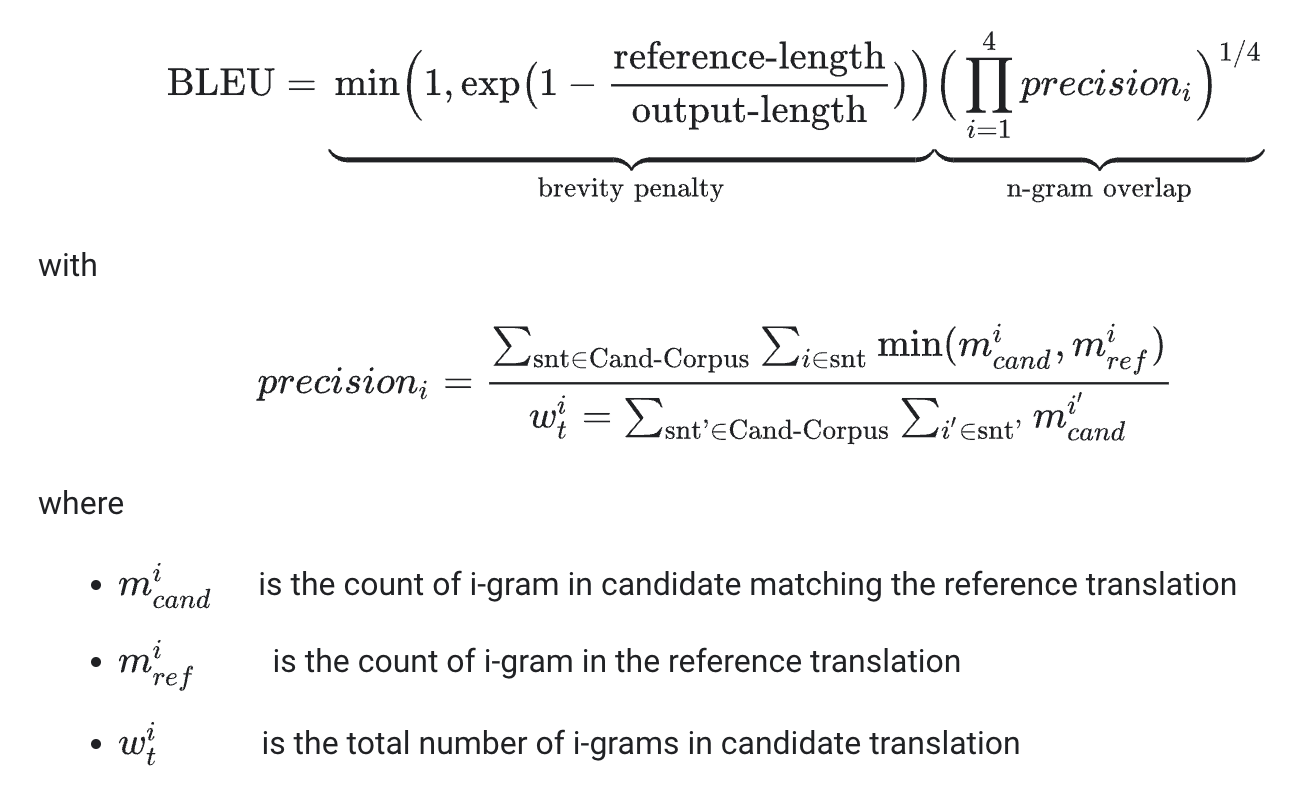
\includegraphics[width=.95\linewidth]{BLEU.png}
    \caption{
        BLEU Formula
    }
    \label{fig:first-page}
\end{figure}
\cite{GoogleBLUE}
\begin{figure}
    \centering
    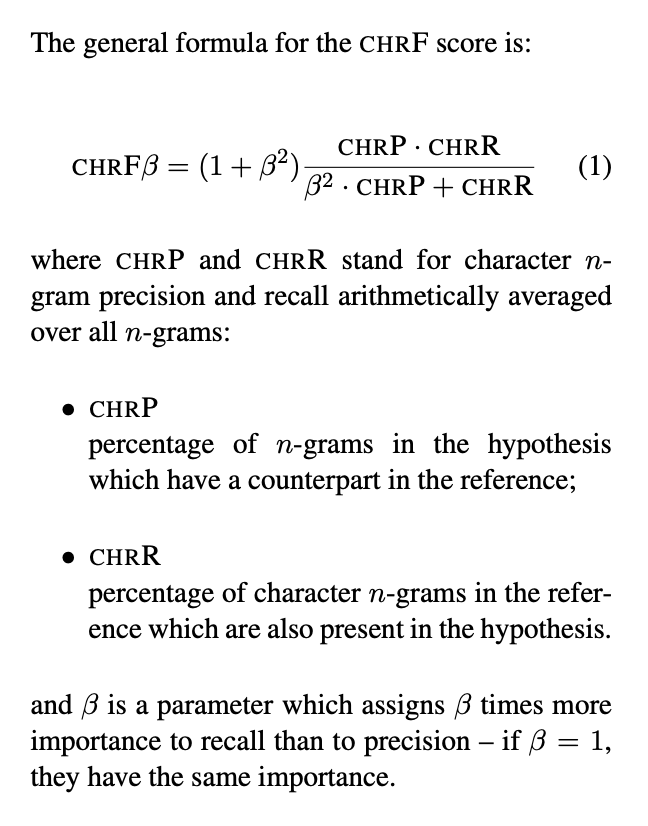
\includegraphics[width=.95\linewidth]{chrF.png}
    \caption{
        ChrF Formula
    }
    \label{fig:first-page}
\end{figure}
\cite{ChrFArticle}

SacreBLEU and chrF both provide scores out of 100, with a higher score indicating a closer match to the reference translation \cite{ChrF} \cite{BLEUGoogle}. 

On the other hand, COMET is a language model trained on human assessments of the semantic similarity and fluency of translations. It calculates a score of from 0 to 1, with a score closer to 1 indicating a closer semantic match and more fluent translations.


SacreBLEU, chrF, and COMET score each translation individually as well as provide an average score for a measure of overall model performance \cite{COMETHF}. I calculated sacreBLEU, chrF, and COMET on 505 Spanish-Nahuatl pairs, which I got from Elotl's Axolotl corpus \cite{Elotl}. 


Automatic evaluation metrics such as SacreBLEU, chrF, and COMET have several drawbacks. SacreBLEU and chrf measure translation quality through comparing predicted translations to reference translations, which means they cannot take into translations that are different but still semantically similar \cite{BLEUCritique}. While COMET is able to take this issue into account, all three metrics provide only numerical scores. They offer no insight into the sources behind mismatches between predicated and reference translations or semantical nonequivalent translations. These shortcomings are why I decided to adopt another evaluation method. 


\section{Feedback from Professor Sousa}
Professor Sousa is a Latin American studies professor who specializes in the Nahua people and their language. After I finished training the models, I asked her to help me evaluate their performance. I compiled three Spanish phrases, their corresponding Nahautl reference translations, and the Nahautl translation each one of my models had produced. I then asked her to look at the Spanish phrase and accompanying reference translation and give me her opinions on them. I wanted examples that my models had translated similarly to the reference, but exactly the same. I used chrF as a guide since it considered the most accurate metric for languages like Nahautl, aiming for phrases than each one of the models had produced a translation scoring between 20 and 60 of. If they had too closely matched the references, there wouldn't be enough variation to discuss what they done correctly and incorrectly. On the other hand, if they were too far off from the reference translation it is possible they would be too incorrect to discuss at all. 


\section{Results}

\subsection{Automatic Evaluation Metrics}


\subsubsection{Training Duration}

\begin{figure}
    \centering
    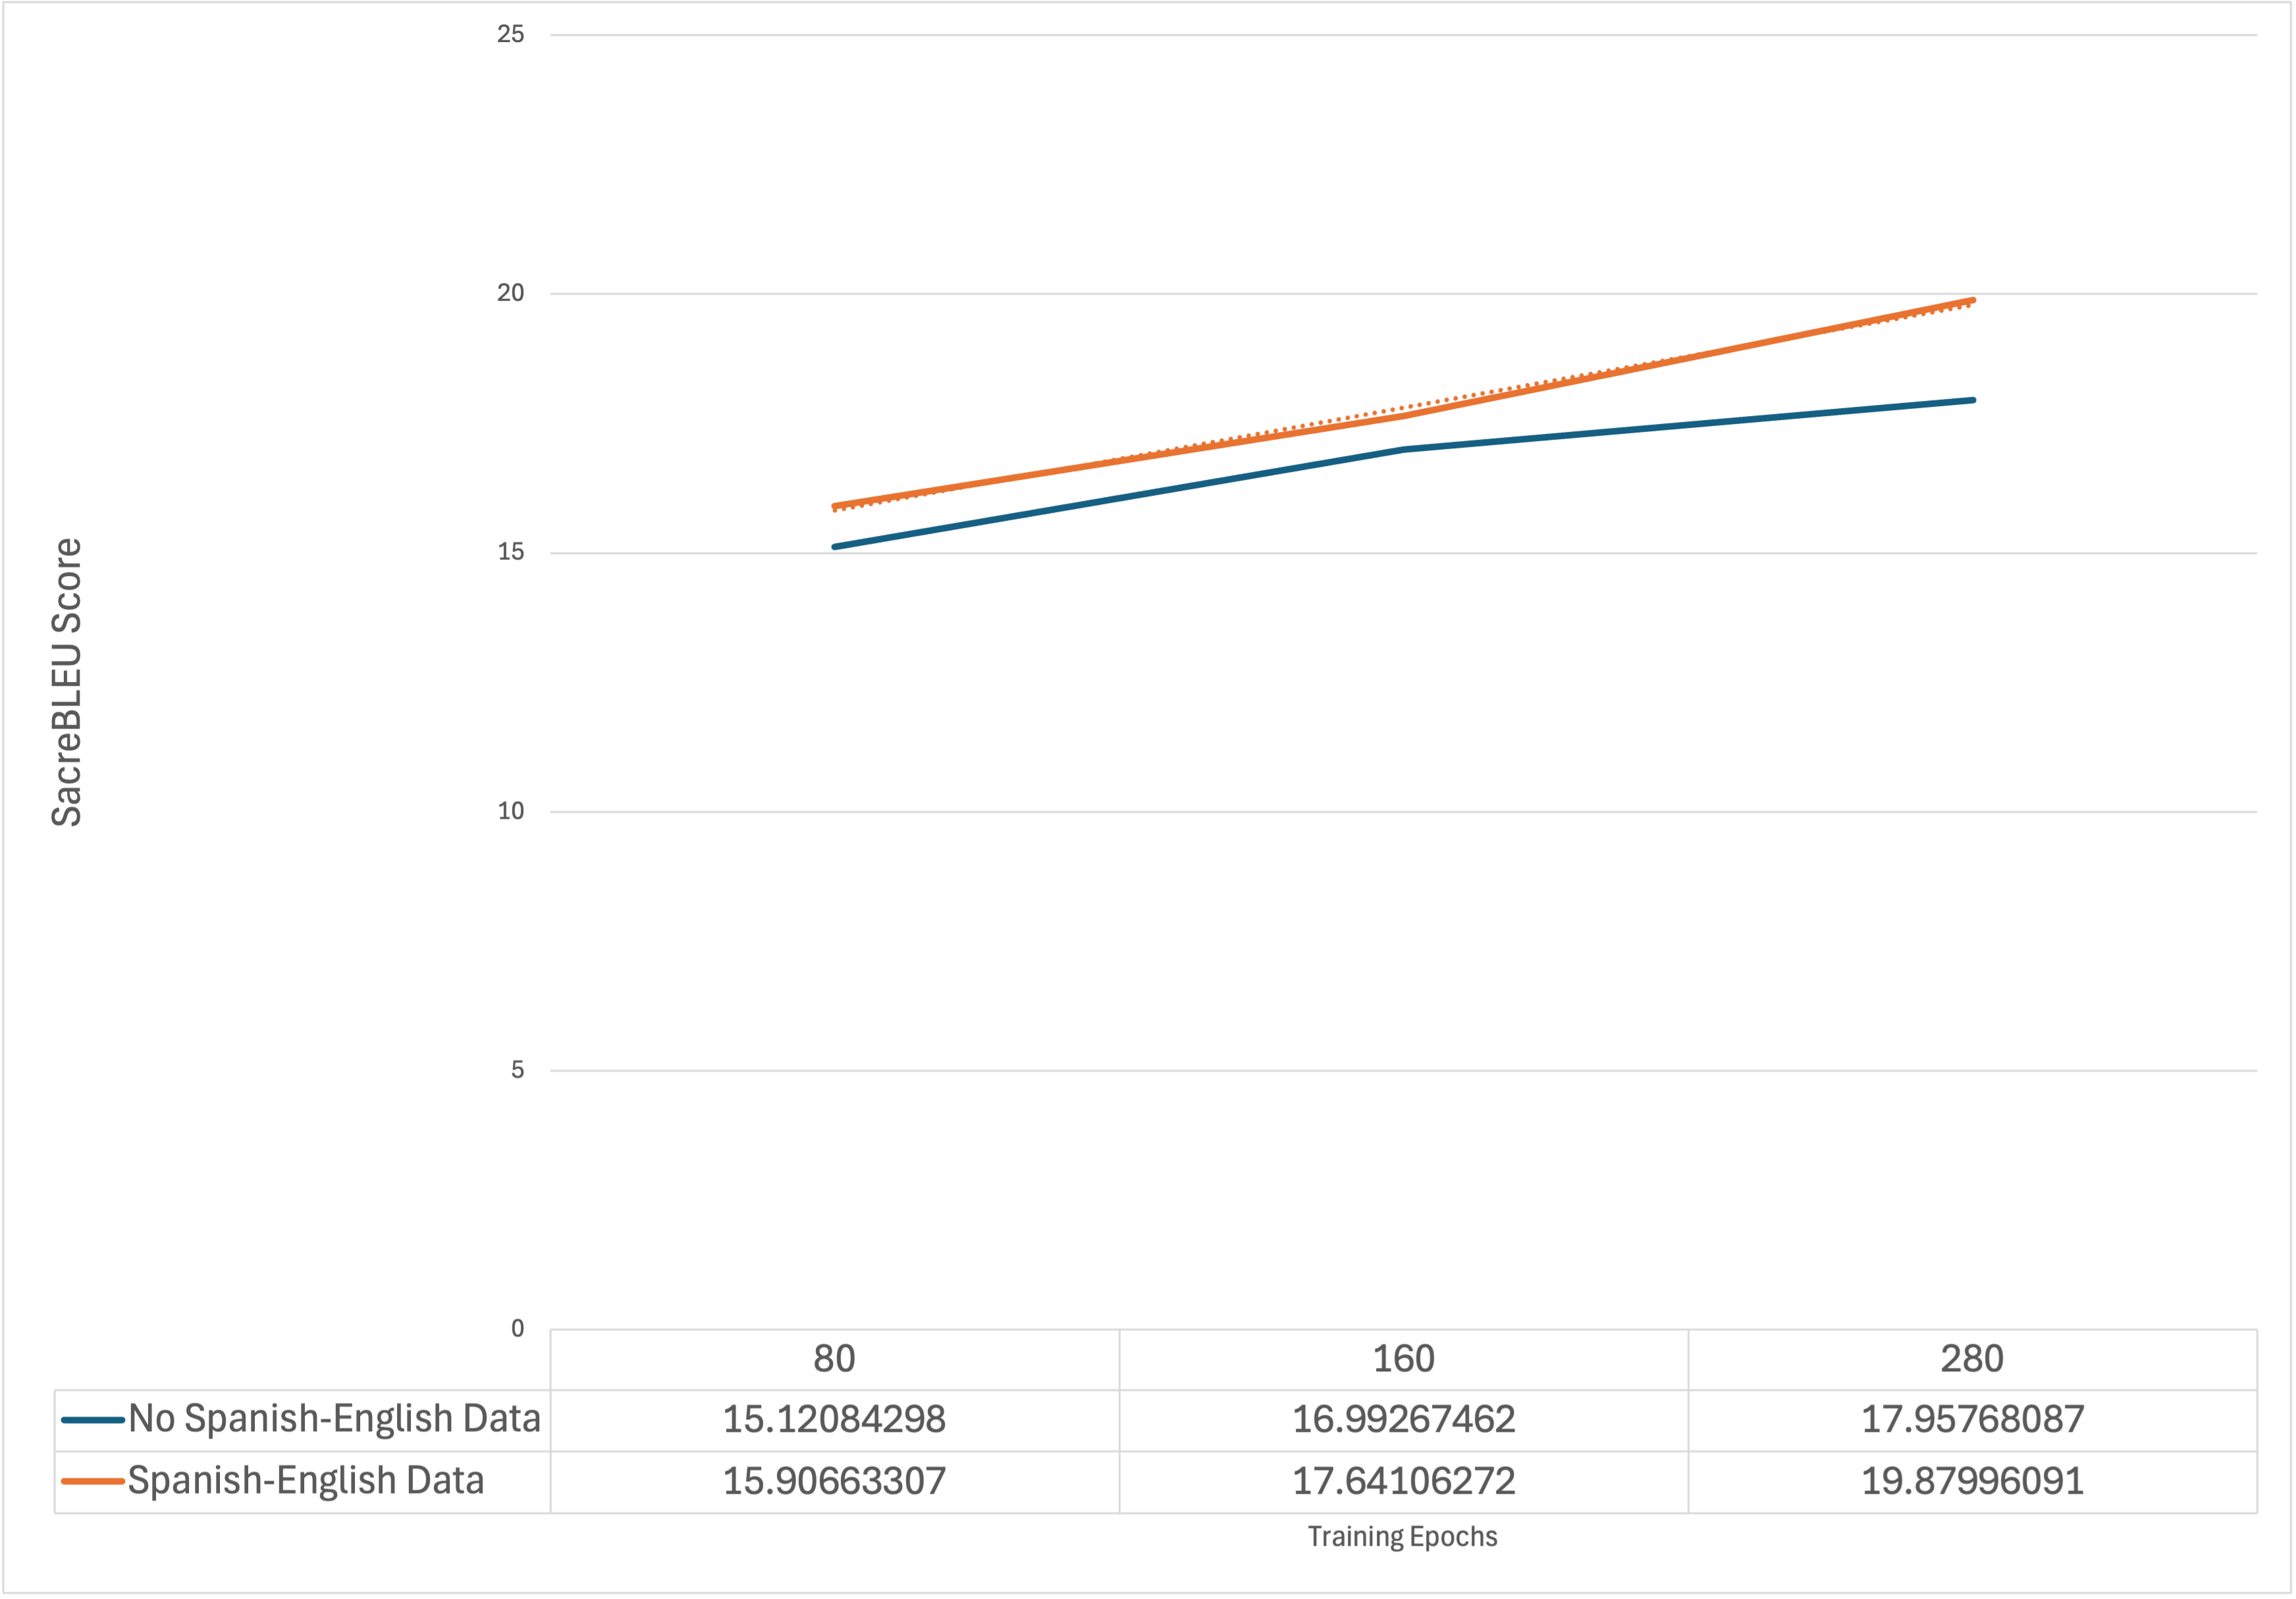
\includegraphics[width=.95\linewidth]{TrainingDurationSacreBLEU.png}
    \caption{
       SacreBLEU score over training duration for model trained with English-Spanish pairs in training data and model trained without English-Spanish pairs in training data
    }
    \label{fig:first-page}
\end{figure}


\begin{figure}
    \centering
    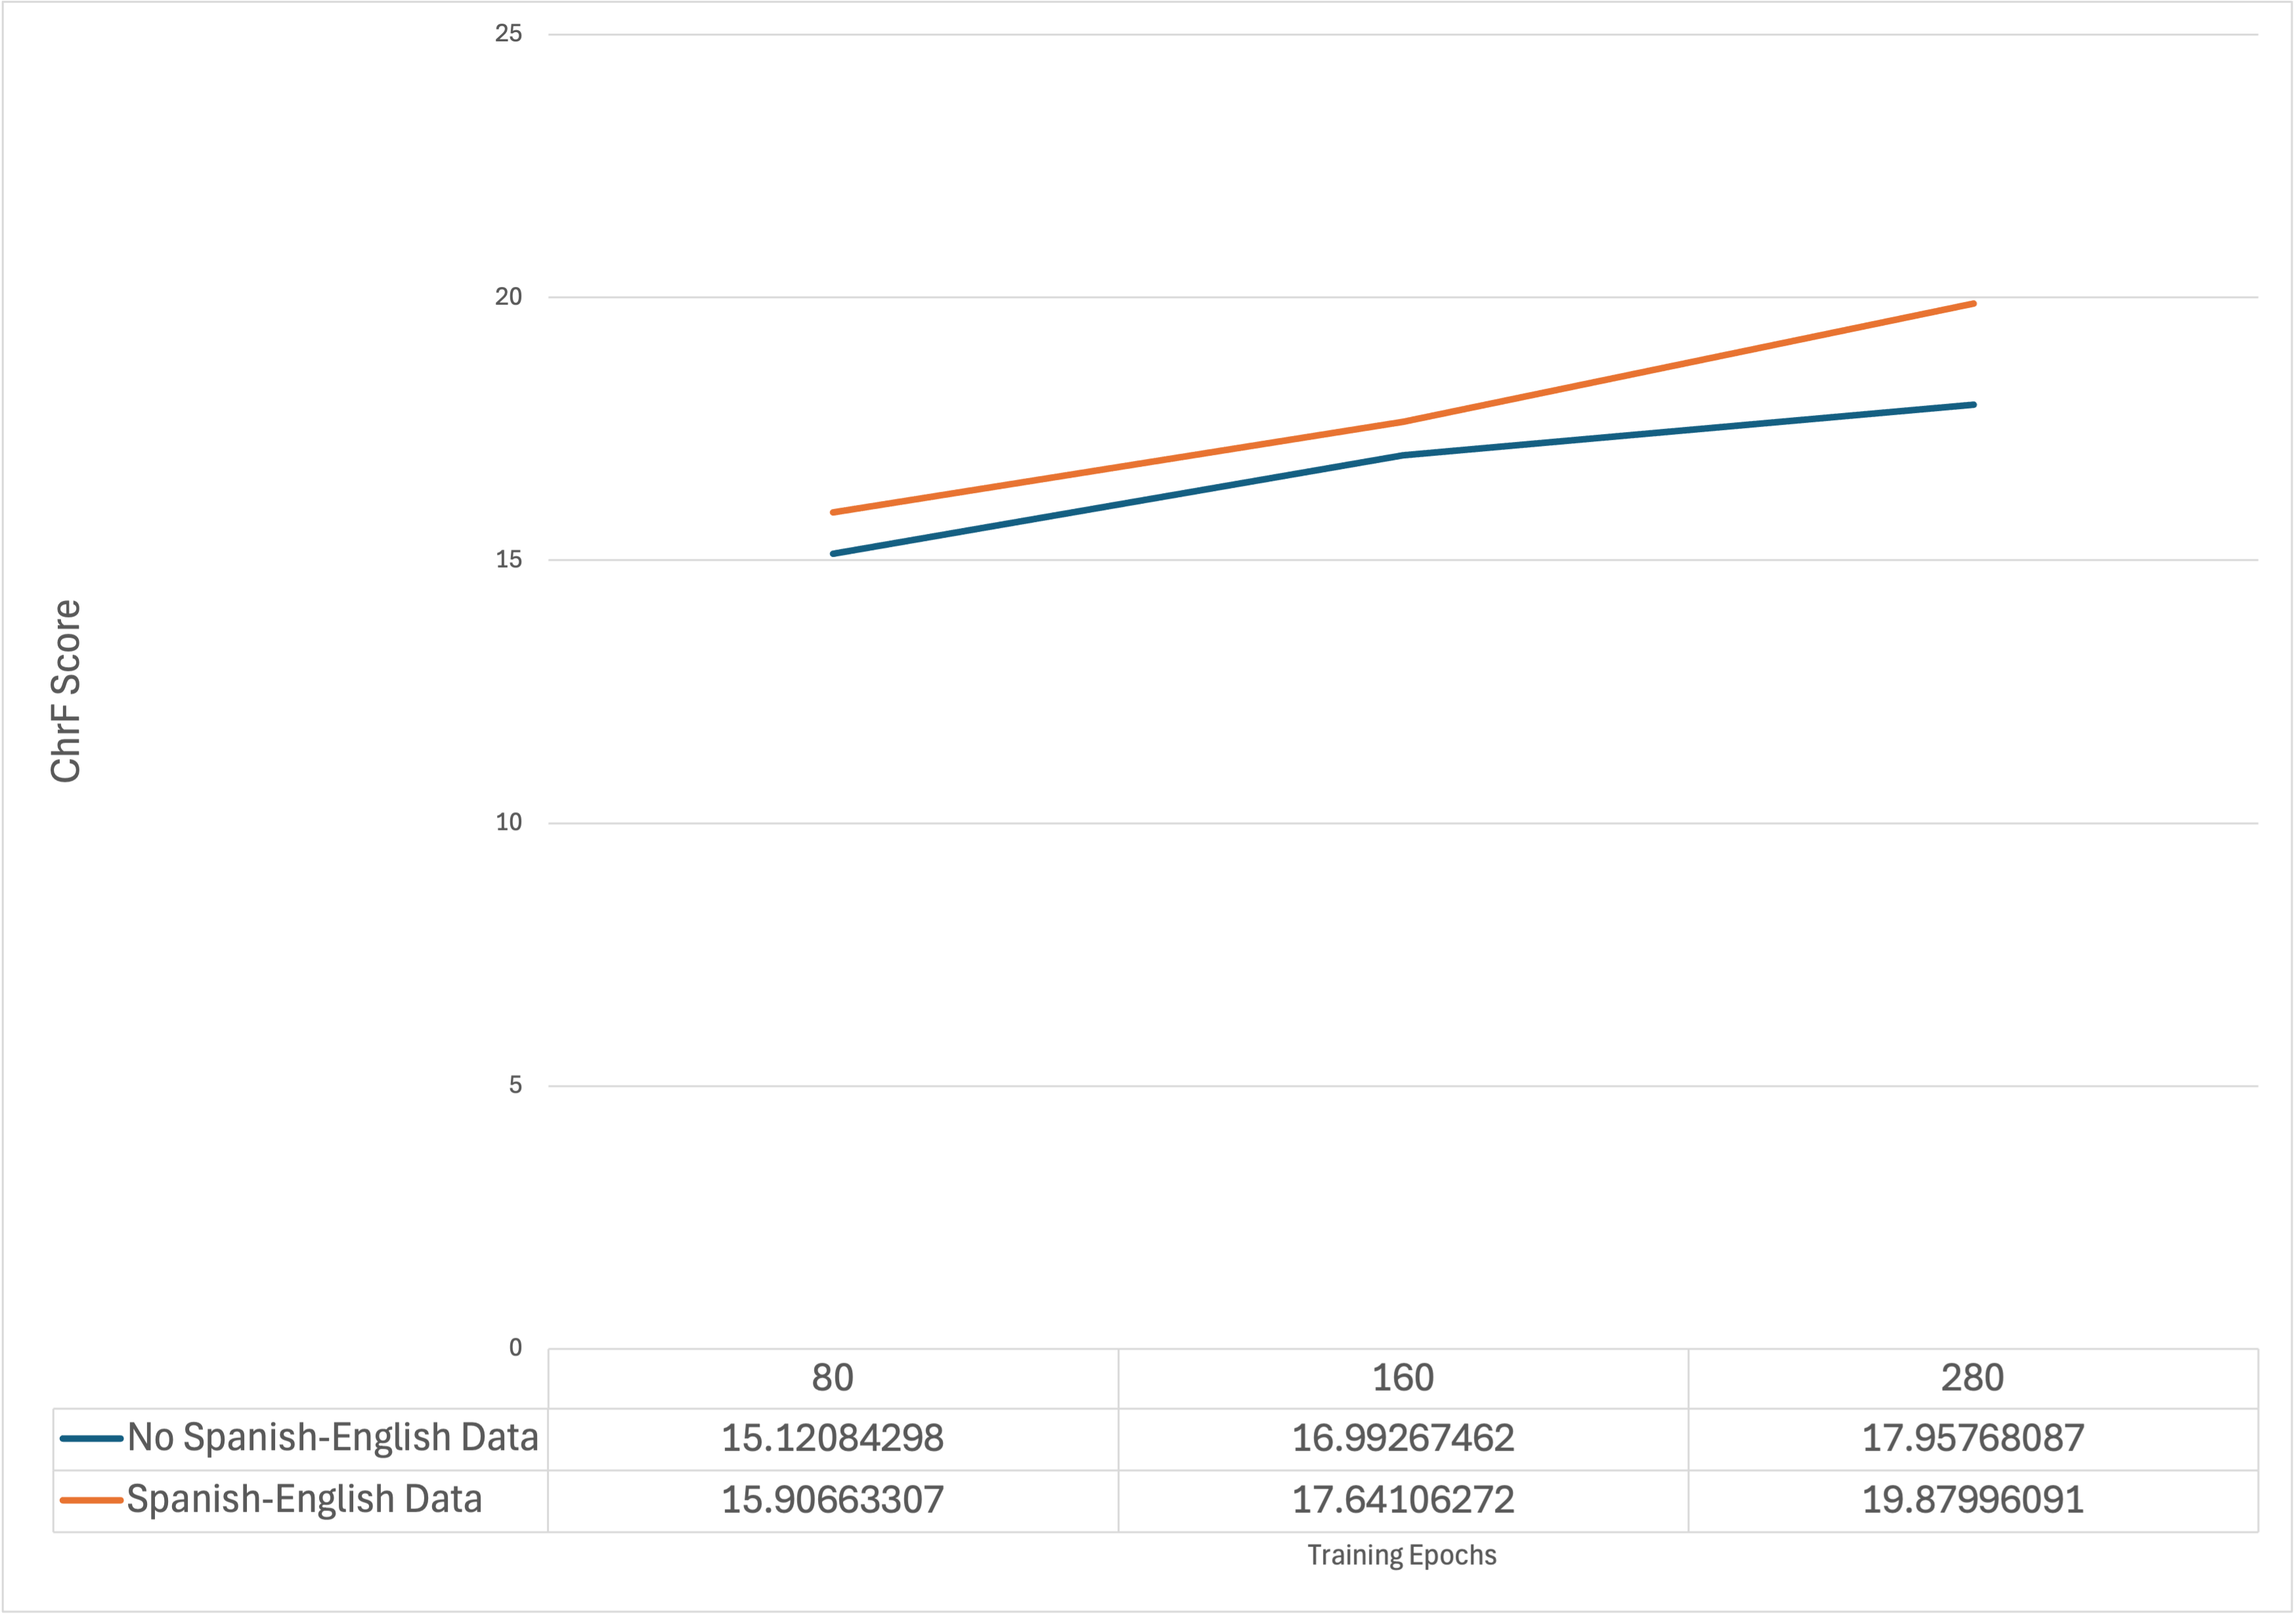
\includegraphics[width=.95\linewidth]{TrainingDurationChrF.png}
    \caption{
        ChrF score over training duration for model trained with English-Spanish pairs in training data and model trained without English-Spanish pairs in training data
    }
    \label{fig:first-page}
\end{figure}


Figures 3 and 4 show how SacreBLEU and chrF scores continue to increase with training duration. COMET scores rise from only 0.516 to 0.530 with English-Spanish pairs in the training data and 0.517 to 0.535 for no English-Spanish pairs, suggesting minimal improvement. 


\subsubsection{English-Spanish Pairs in Training Data}
The model trained with English-Spanish pairs in the training data achieves a sacreBLEU score of 3.859 and a chrF score of 19.878 while the model with no English-Spanish pairs achieves scores of 3.190 and 17.958. There is minimal difference in COMET scores (0.529 to 0.535). 


\subsubsection{Orthography Normalizer}

\begin{figure}
    \centering
    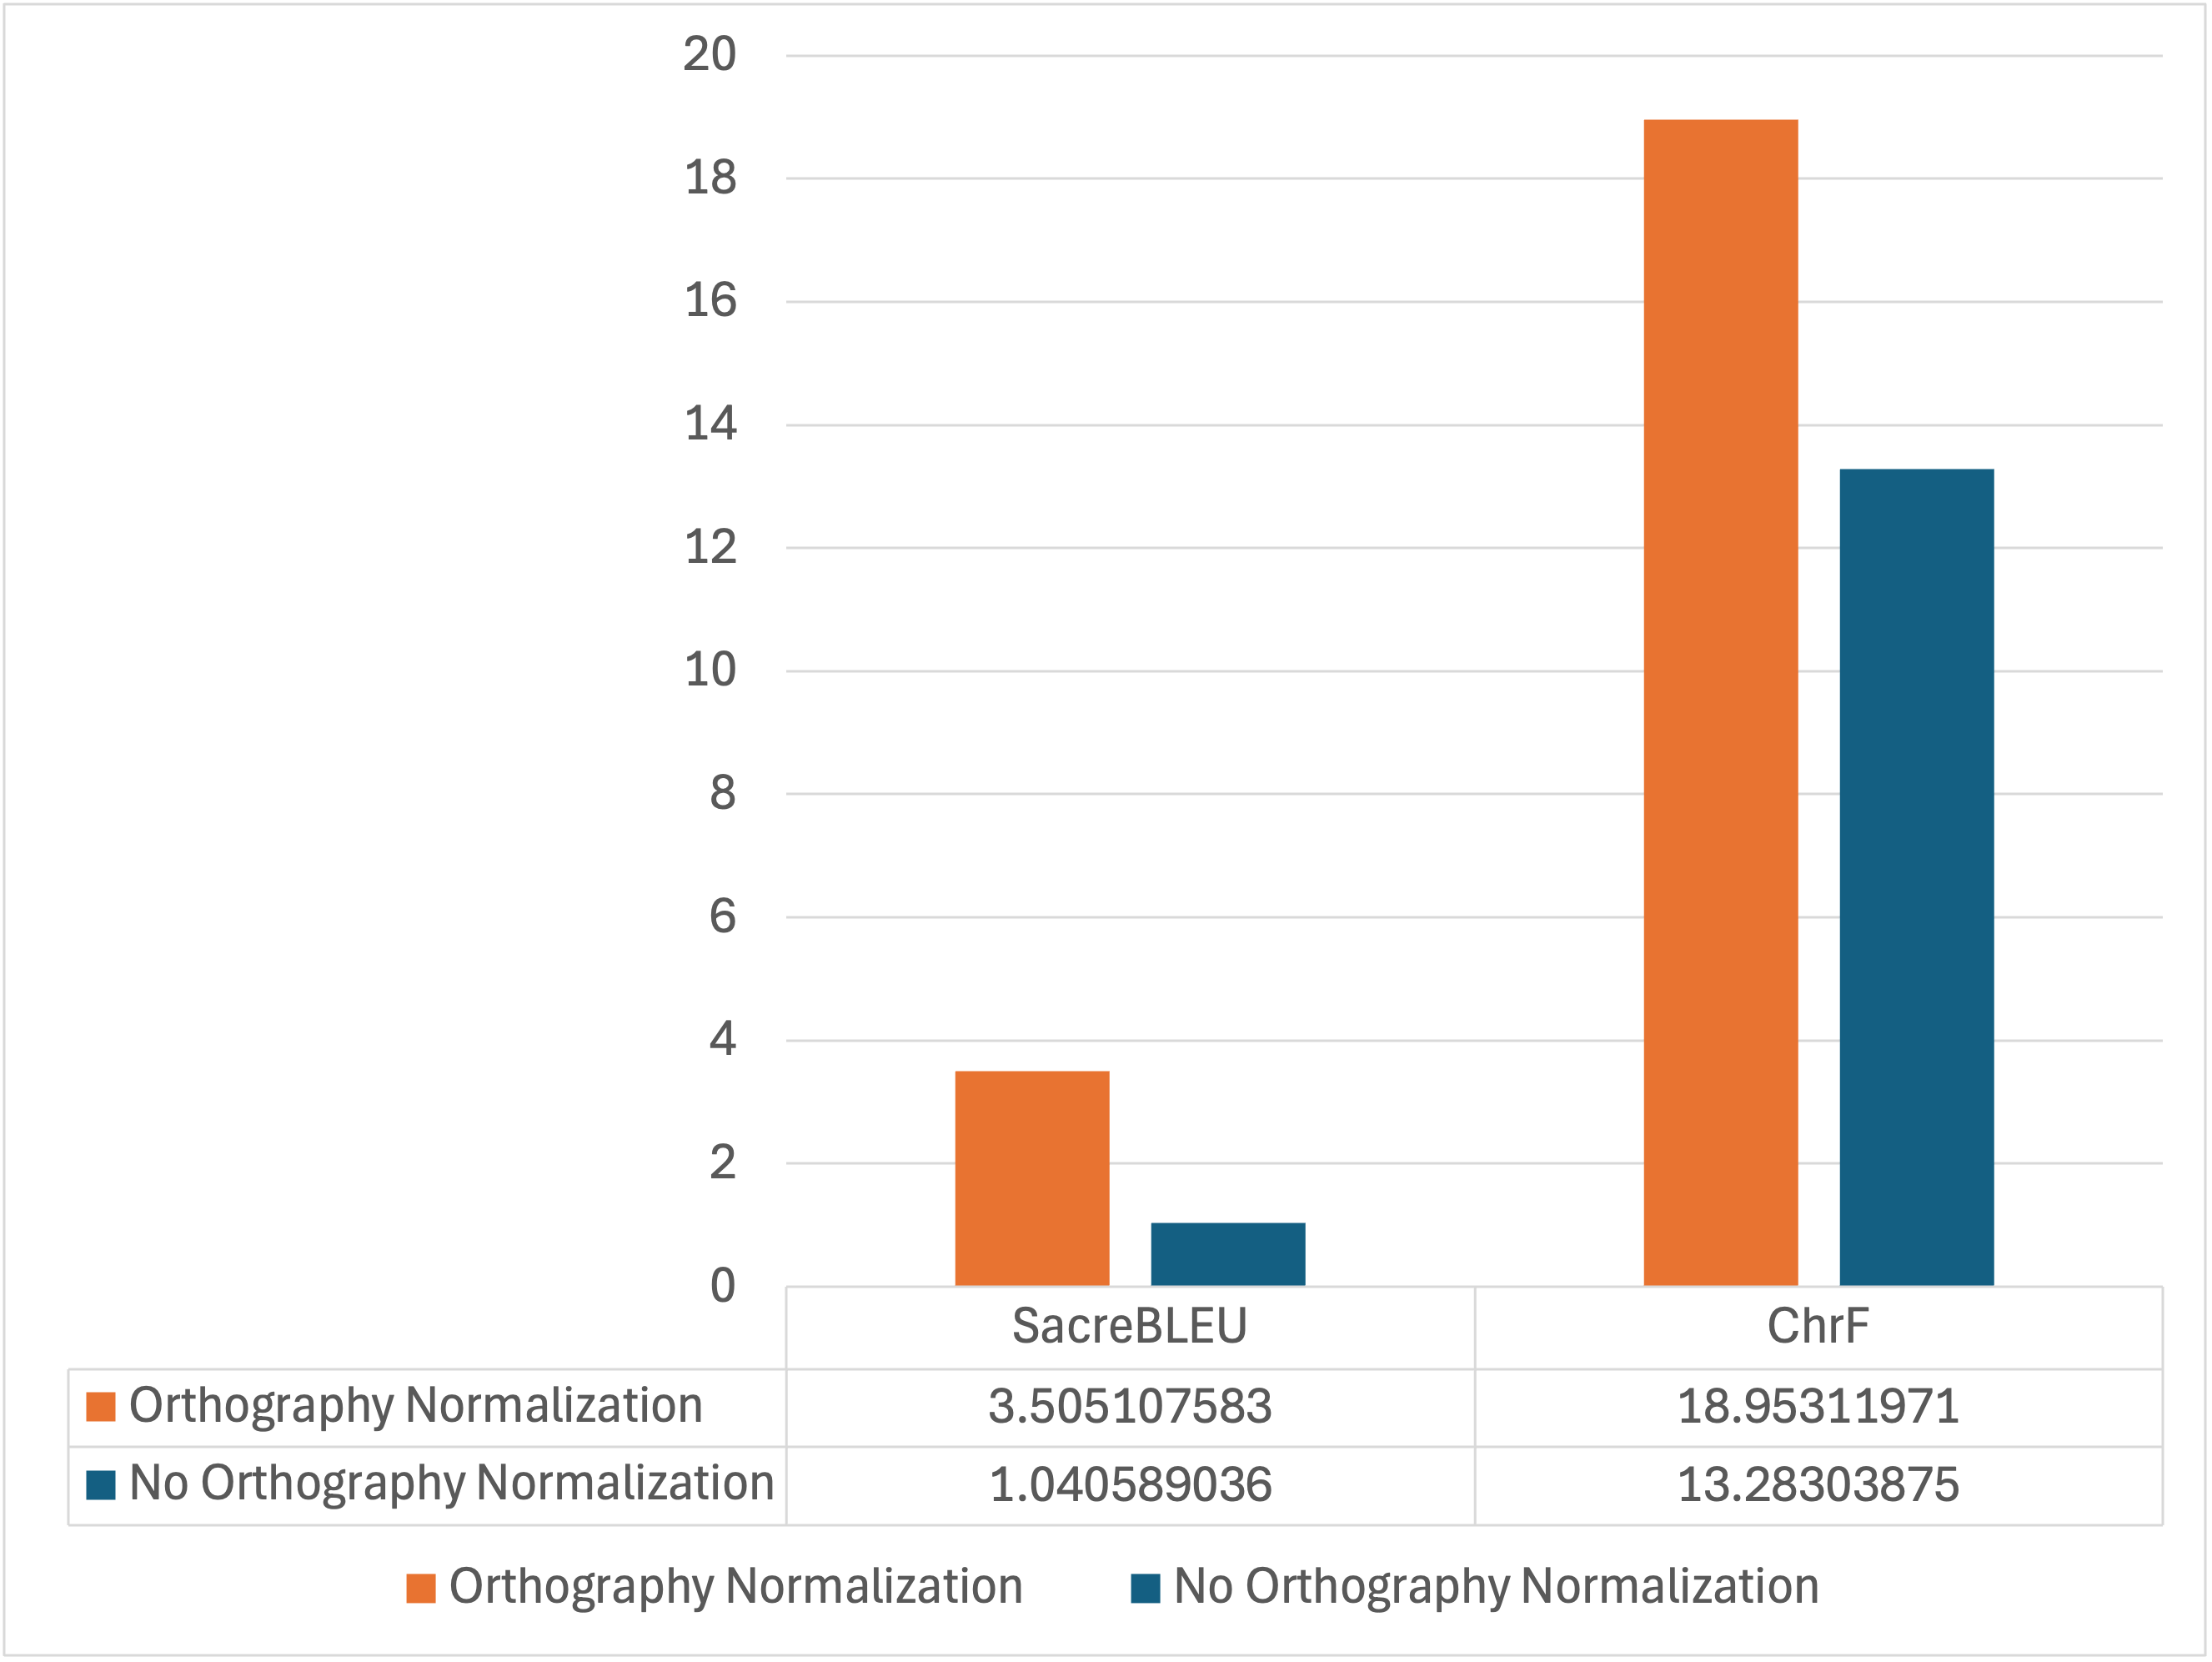
\includegraphics[width=.95\linewidth]{Orthography.png}
    \caption{
        SacreBLEU and chrF scores for model trained on orthographically normalized data vs. model trained on non orthographically normalized data
    }
    \label{fig:first-page}
\end{figure}

Figure 5 shows the model trained on orthographically normalized data achieves higher sacreBLEU and chrF scores. It also achieves a higher COMET score 0.529 compared to 0.495.


\subsubsection{Modern vs. Modern and Classical Data}

\begin{figure}
    \centering
    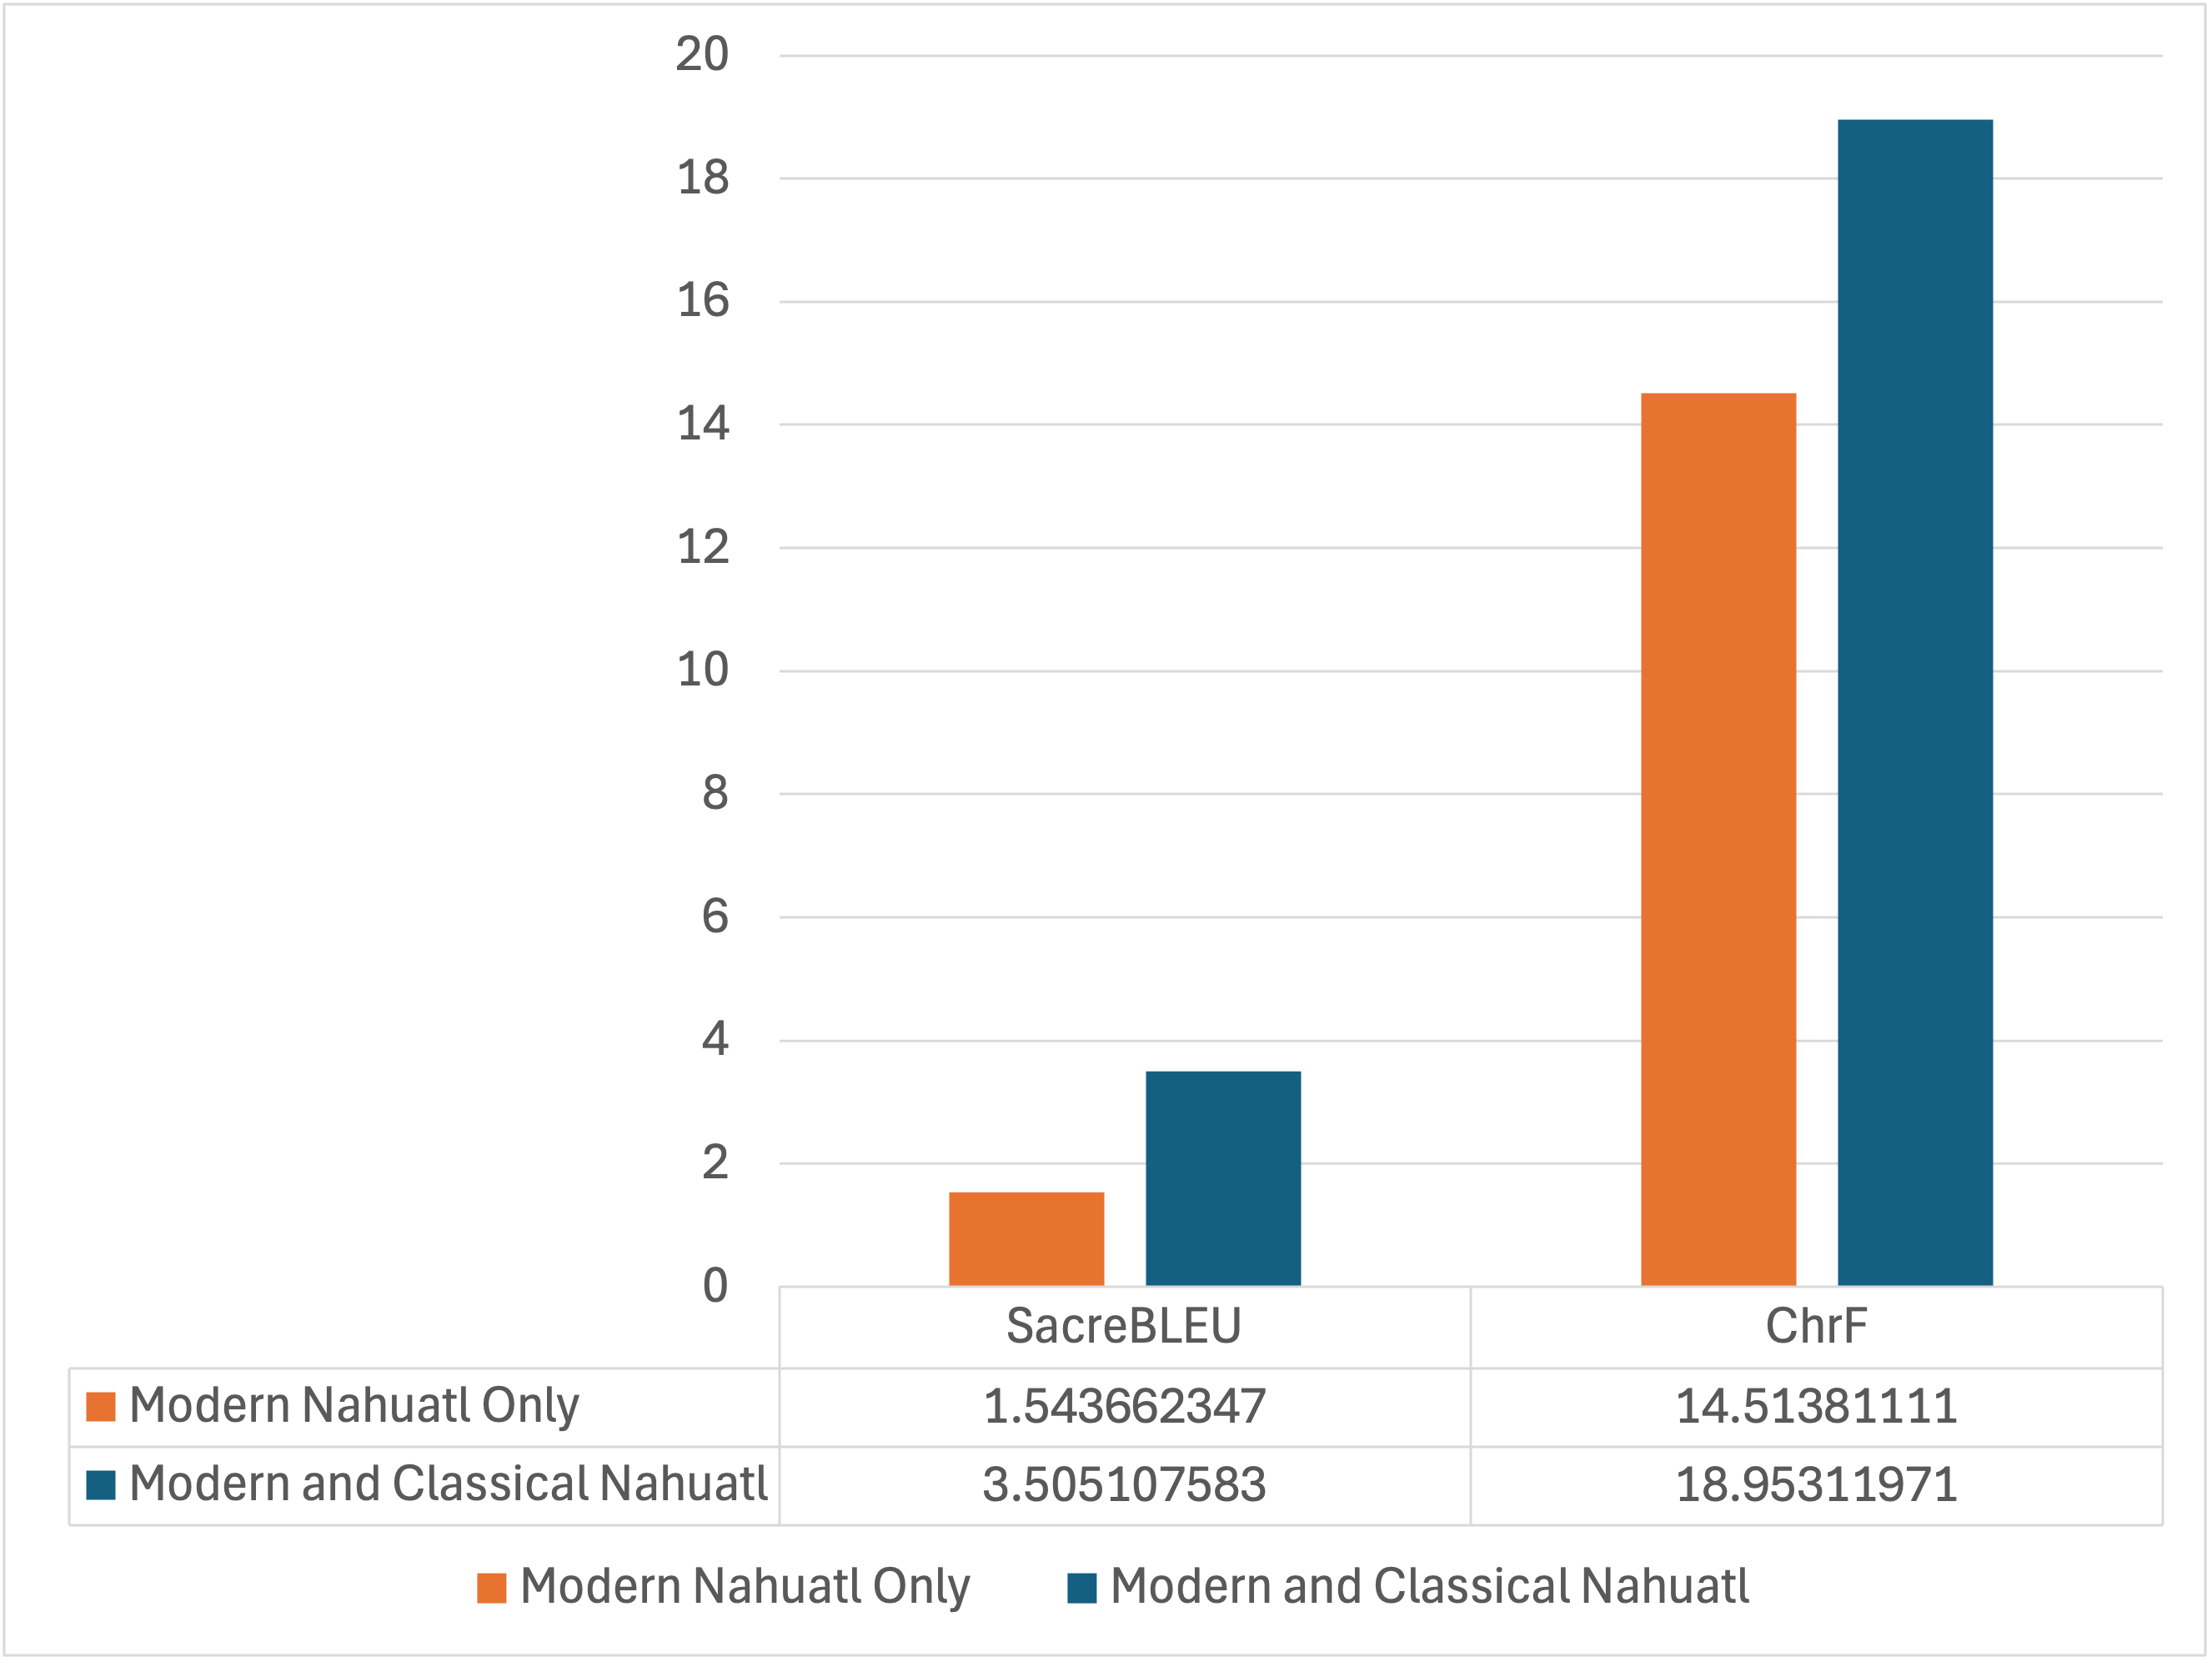
\includegraphics[width=.95\linewidth]{Dialect.png}
    \caption{
        SacreBLEU and chrF scores for model trained on data featuring only modern Nahuatl vs. both modern and classical
    }
    \label{fig:first-page}
\end{figure}

Figure 6 show the model trained on data featuring both modern and classical data achieves higher sacreBLEU and chrF scores than the model trained on data featuring only modern data. It also achieves a higher COMET score (0.533 to .509).

\subsubsection{Cross-lingual Pretraining}
\begin{figure}
    \centering
    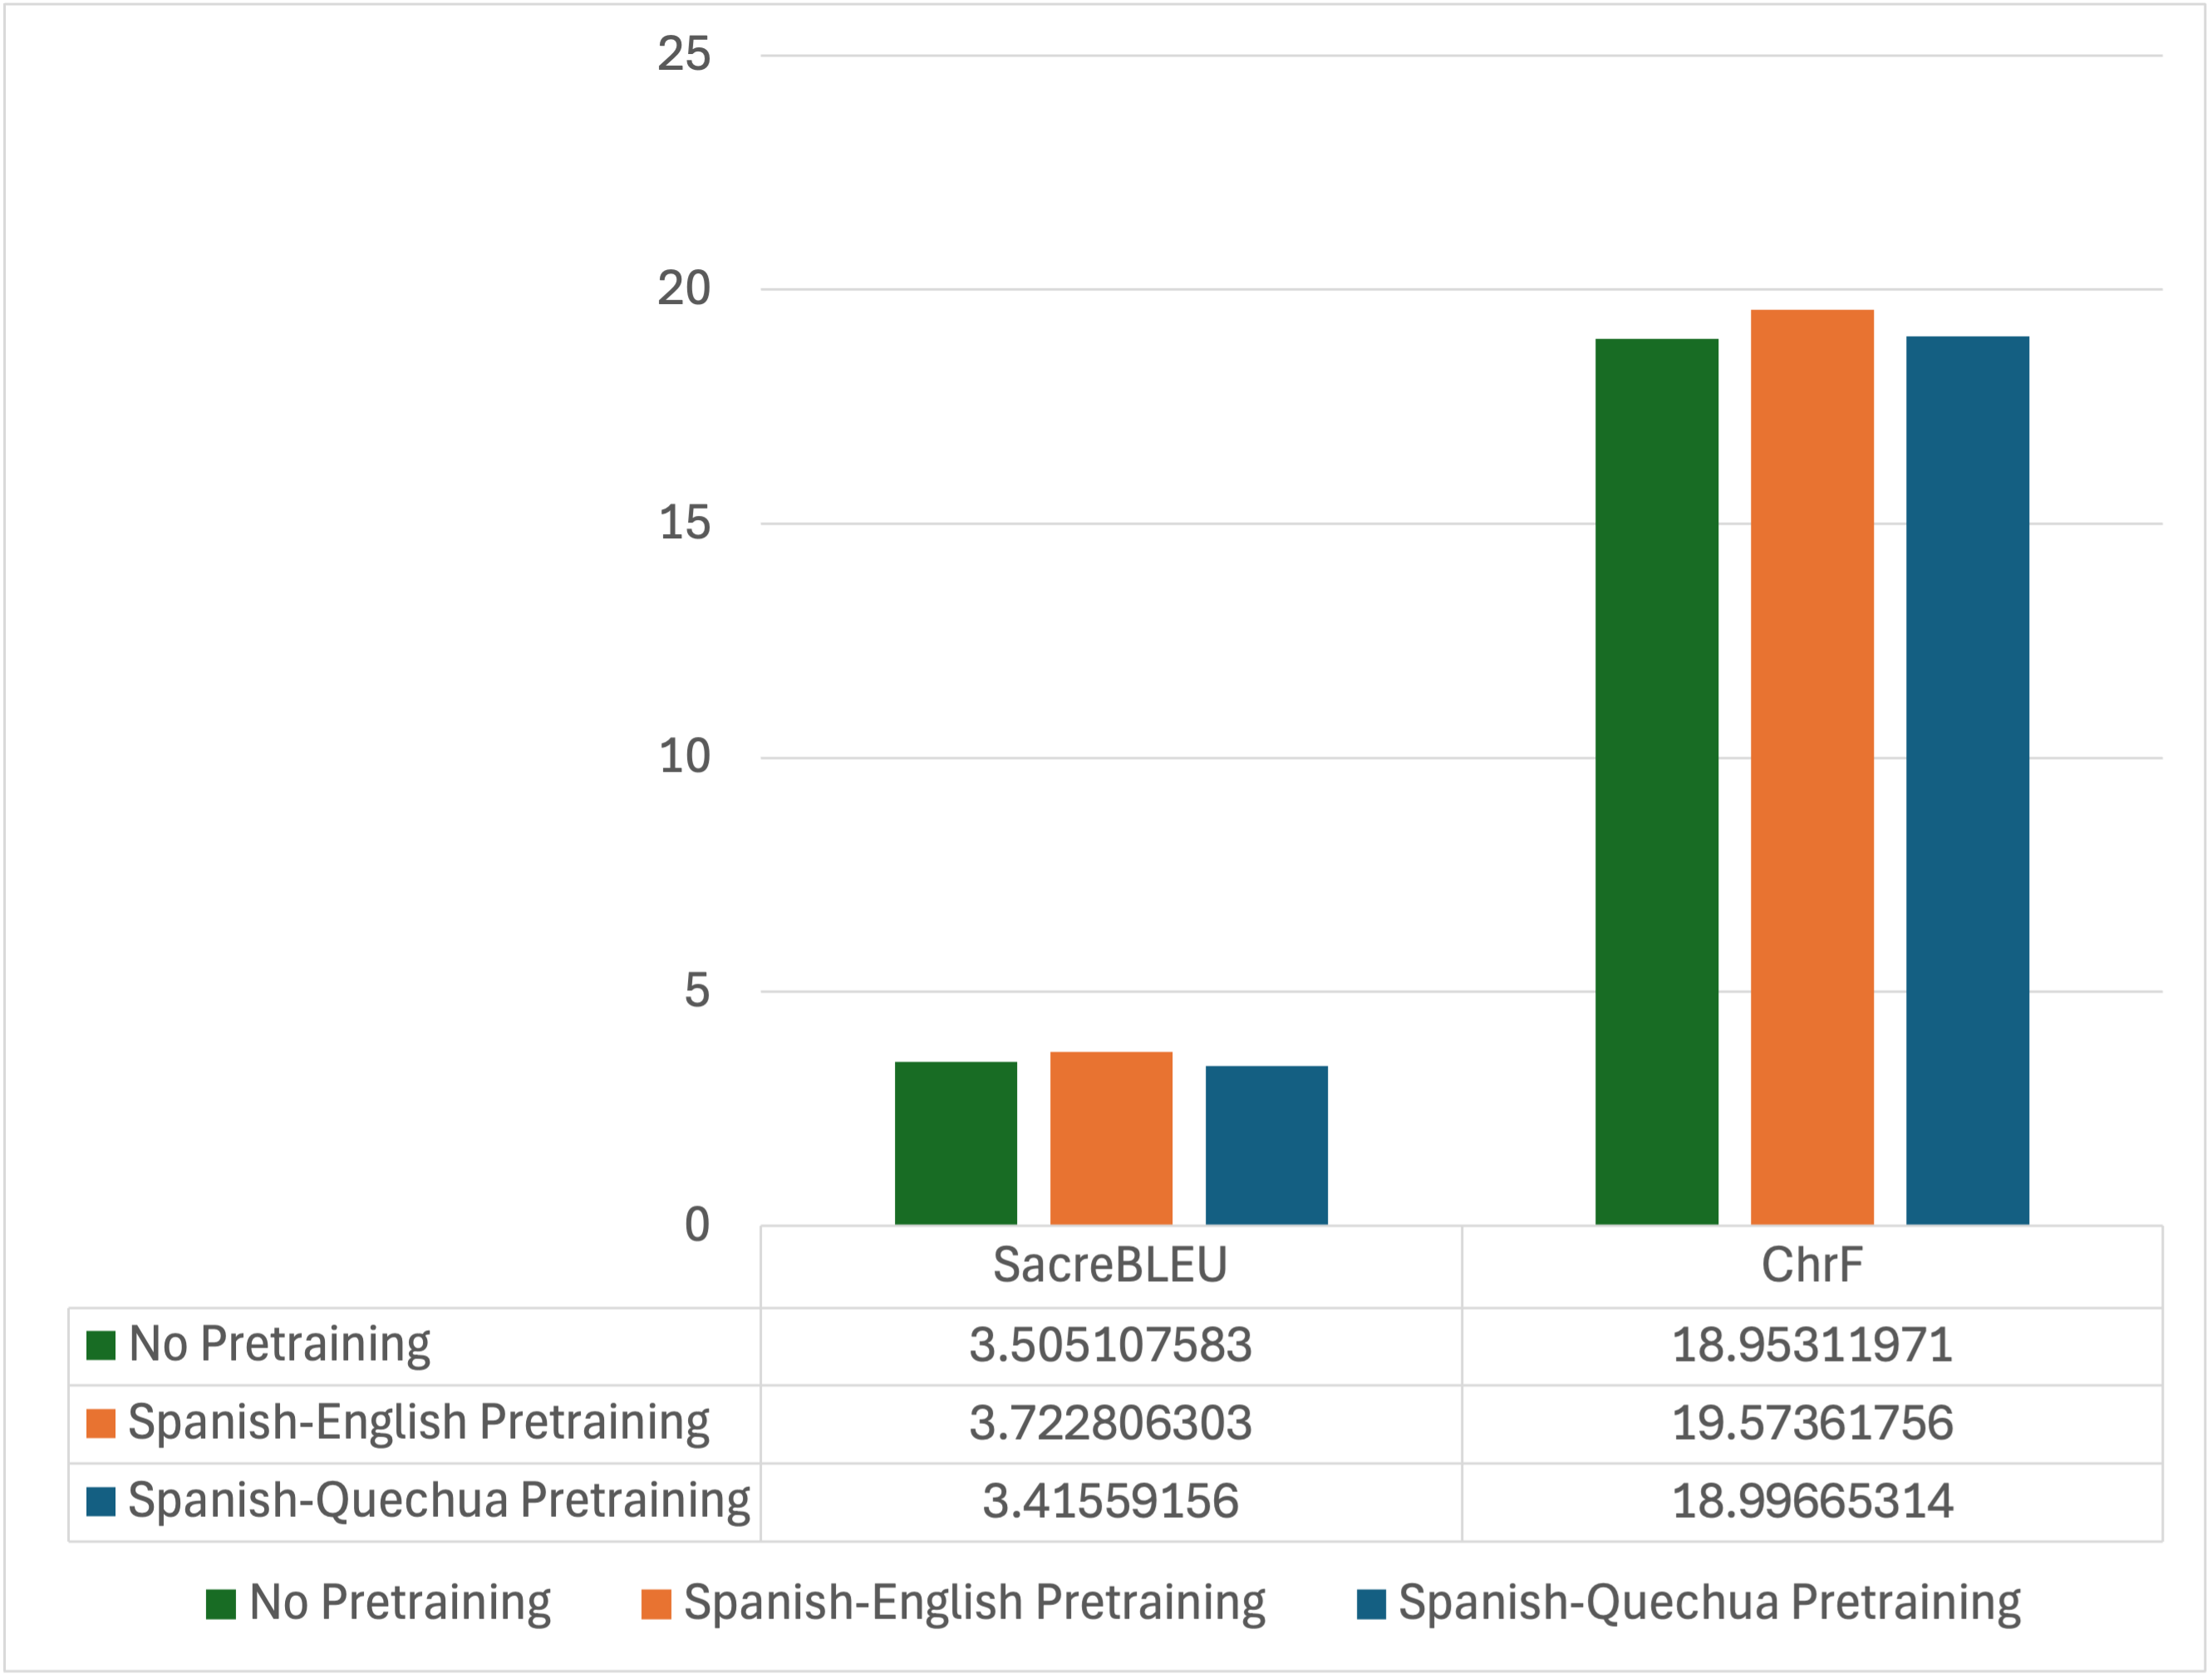
\includegraphics[width=.95\linewidth]{Pretraining.png}
    \caption{
        SacreBLEU and chrF scores for Spanish-English pretrained model, Spanish-Quechua pretrained model, and model not pretrained
    }
    \label{fig:first-page}
\end{figure}
Figure 7 shows the two pretrained models achieve higher sacreBLEU and chrF scores. However, COMET score is only slighly higher (0.533 to 0.529). The difference in scores between the language pairs is minimal. 

\subsection{Feedback from Sousa}
For each set of examples I brought to Professor Sousa, I include the Spanish prompt, its accompanying Nahuatl reference translation,  the translations generated by my models listed from highest to lowest chrf score, and Professor Sousa's feedback.

Example 1: \\
    Spanish prompt: \textit{Florea todo el tiempo} \\
    Nahuatl reference translation: \textit {Nochipa xochiyojtok} \\
    Nahuatl translations produced by my models:
    
\begin{enumerate}
    \item Model pretrained in Spanish-English: \\
    Predicted translation: \textit{Xochiyoua nochi tonajli} \\ ChrF score: 46.2151556384343
    \item Model trained with English-Spanish pairs in training data: \\
    Predicted translation: \textit{xochiyoua nochi tonali} \\ ChrF score: 45.8650904067153
    \item Baseline: \\
    Predicted translation: \textit{xochiyoua nochi tepetl}\\ ChrF score: 44.907231215831
    \item Model pretrained in Spanish-Quechua: \\
    Predicted translation: \textit{xochiyoua nochi tlakatl.} \\ ChrF score: 43.84991501
    \item Model trained on data not normalized orthographicly: \\
    Predicted translation: \textit{Nochi in xochiyoua in totonik} \\ ChrF score: 40.15858
    \item Model trained on data featuring only modern Nahuatl: \\
    Predicted translation: \textit{nochi tlakatl yejuan tlakuajt}. \\ ChrF score: 18.90334 
\end{enumerate}

Sousa's Feedback:
Sousa indicated the model pretrained in Spanish-English and the model trained with English-Spanish pairs produces the most accurate translations for the prompt. While the reference translation roughly translates to "it is always blooming", the translation generated by these two models is closer to "it blooms every day". According to Professor Sousa, this is a different but still correct way of translating the prompt. She also notes that the translation produced by the model trained on only modern Nahautl data is unintelligible and the least accurate translation. 


Example 2: \\ 
    Spanish prompt: \textit{Sus hojas son medicinales} \\
    Nahuatl reference translation: \textit{ixiuyo no pajti} \\
    Nahuatl translations produced by my models: \\

\begin{enumerate}
    \item Baseline: \\
    Predicted translation: \textit{ixiuyo pajti} \\ ChrF score: 64.0623211584073
    \item Model pretrained in Spanish-English: \\
    Predicted translation: \textit{ixiuyo kikuaj pajti} \\ ChrF score: 49.6157404787726
    \item Model trained with  English-Spanish pairs in training data: \\
    Predicted translation: \textit{ixiuyo kualtia para pajti} \\ ChrF score: 45.8015176279116
    \item Model pretrained in Spanish-Quechua: \\
    Predicted translation \textit{tein kualtia para pajti} \\ ChrF score: 23.96020542
    \item Model trained on data featuring only modern Nahuatl: \\ 
    Predicted translation: \textit{in tlajtoli tlakuali} \\ ChrF score: 14.66797
    \item Model trained on data not normalized orthographically: \\ 
    Predicted translation: \textit{In tepitzin} \\ ChrF score: 6.72043
    
\end{enumerate}

Sousa's feedback:
Sousa indicated the baseline model produces the best translation. While both the reference translation and the baseline model's translation can be roughly translated to English as "the leaves are medicine", the translation produced by the model trained with English-Spanish pairs in the training data can be translated to English as "the leaves are good for medicine". It uses the Spanish word \textit{para} for "for". Thus, it not only adopts a different structure but uses a Spanish word. 


Example 3: \\
    Spanish prompt: \textit{Su semilla se siembra como la de las anonas} \\
    Nahuatl reference translation: \textit{se kitoka iteyo kemej kanones} \\
    Nahuatl translations produced by my models: \\
\begin{itemize}
      \item Model pretrained in Spanish-English: \\ 
    Predicted translation: \textit{iteyo se kitoka ken iuan anonas.} \\ ChrF score: 43.5016752463149
    \item Baseline: \\ 
    Predicted translation: \textit{in iteyo se kitoka ken ipan anonas} \\ ChrF score: 42.7788026148408
     \item Model pretrained in Spanish-Quechua: \\
    Predicted translation: \textit{in iteyo se kitoka ken se ikuitlapan} \\ ChrF score: 39.62059634
    \item Model trained on data not orthography normalization: \\ 
    \item Model trained with  English-Spanish pairs in training data: \\ 
    Predicted Translation: \textit{iteyo se kitoka ken iteyo tepits} \\ ChrF score: 39.283941067485
    Predicted translation: \textit{In iteyo on tetl yejhuan} \\ ChrF score: 18.79408
    \item Model trained on data featuring only modern Nahuatl: \\ 
    Predicted translation: \textit{niman ijkuak yotlakuaj ken on} \\ ChrF score: 16.22464
\end{itemize}

Sousa's feedback:
Sousa had difficulty understanding any of the translations for this prompt. She does note, however, that both the model pretrained in Spanish-English use the Spanish word \textit{se} in their predicted translations. It appears using Spanish words in the Nahuatl translations isn't exclusive to the model trained with English-Spanish pairs in the training data.

\section{Discussion}
\subsection{Training Duration}
Evaluation metric scores continue to increase for both models even at 280 epochs, indicating a long training training does improve model performance. However, chrF and sacreBLEU increase incredibly slowly, showing this is not the most efficient method to improve results.

\subsection{English-Spanish Pairs in Training Data}
The model trained with English-Spanish data achieves higher sacreBLEU and chrF scores. However, I don't feel confident saying this reflects an improvement in performance. In my discussion with Professor Sousa, she pointed out how this model used the Spanish word \textit{para} in its translation and deviated heavily from the reference, attempting to produce a translation that conveyed "the leaves are good for medicine" instead of "the leaves are medicine". While translations don't have to perfectly match references to be accurate and fluent, this translation expresses a different idea than the prompt and reference. However, Sousa did pick out its translation of \textit{florea todo el tiempo} as among the most accurate. In conclusion, I do not feel confident saying this technique improves or worsens performance. I believe more analysis and experimentation is needed.

\subsection{Orthography Normalizer}
The model trained on data that has been orthographically normalized achieves higher sacreBLEU, chrF, and COMET scores. Additionally, Sousa picks out a translation produced by the model trained on non normalized data as among the least accurate for all three examples. This clearly indicates that having a consistent orthography improves performance for Spanish-Nahautl translation. 

\subsection{Modern vs. Modern and Classical Data}
The model trained on data featuring only modern Nahautl receives lower sacreBLEU, chrF, and COMET scores. It is clear that when data is this scarce, quantity is more important than consistency. 

\subsection{Cross-lingual Pretraining}
Both pretrained models achieve higher sacreBLEU, chrF, and COMET scores, reaching some of the highest scores out of any of the models. Interestingly, the Spanish-English pretrained model performs slightly better, despite Quechua being more similar to Nahautl than Spanish is. Sousa's feedback affirms this, with her pointing out one of the translations produced by the Spanish-English pretrained model as among the most accurate and not any from the Spanish-Quechua pretrained model. 

I suspect the model was able to learn to translate Spanish more effectively than it was Quechua, since T5 comes trained on several languages that are much more similar to Spanish. This would indicate that mastering the pretraining language is more important than picking a language that is similar. 

These results indicate that cross-lingual pretraining does improve performance. However, they suggest picking a linguistically similar language for pretraining may not be important, although further research is needed to determine this. 

\subsection{Takeaways}
Overall, Spanish-Nahuatl ML-based translation can be improved through cross-lingual pretraining and orthography normalization. However, my results indicate the choice of language pair may not be important, although more research is needed. Additionally, it remains unclear if adding English-Spanish data is an effective strategy. Lastly, due to the limits of automatic evaluation metrics, human feedback is necessary to get a more complete understanding of model performance.


\section{Ethical Considerations}
    The primary ethical concern my project presents stems from my identity and how it relates to that of the people who speak Nahuatl. Nahuatl is an indigenous language of present day Mexico. I am not a part of any indigenous group or culture, meaning I am considered a non-indigenous researcher. Unfortunately, non-indigenous researchers can and have caused significant harm to the communities their work relates to. 

Non-indigenous researchers have refused to take input on research methodologies, spread harmful western ideologies, and acted in a self-serving manner, ultimately causing research’s legacy in indigenous communities to be one of harm. Simmons and Christopher (2013) \cite{AdaptingWesternMethods} explain how indigenous research methodologies can differ from other approaches, especially from traditional western ones. However, researchers have often refused to adapt their methods and disrespected cultural norms in the process. Additionally, research has resulted in the spread of harmful western ideologies in communities. For example, researchers have imparted their own racist views on group members, reinforcing internalized racism in the community \cite{TalkAboutWhatYouDontKnow}. Simmons and Christopher (2013) \cite{AdaptingWesternMethods} also explain how researchers have entered communities with the sole aim of furthering their own careers, using indigenous cultures and people for personal gain. It is no surprise then that the legacy of research in indigenous communities is one of harm. As Maori scholar Linda Tuhiwai Smith once described said, research is one ”one of the dirtiest words in the indigenous world’s
vocabulary” \cite{VingnettesAsAStrategy}.

Unfortunately, even well-meaning researchers can cause harm because of how different their cultural background is. Indigenous communities have different cultural norms, which are easy for researchers to disrespect if they do not take the time to understand the community they are working in \cite{TalkAboutWhatYouDontKnow}. Additionally, indigenous people can have profoundly different ways of understanding the world. For example, indigenous and western researchers have deep epistemological differences regarding concepts such as land and the environment \cite{TalkAboutWhatYouDontKnow}. To genuinely understand the community they are operating in, researchers must again put significant effort into getting to know how they understand the world. In conclusion, even well meaning researchers can cause harm to indigenous communities if they don’t work to understand their culture and views.

 Non-indigenous researchers can cause harm to comminutes, even unintentionally through ignorance. My plain to mitigate these concerns involved learning about the language and culture through taking  Professor Sousa's  Nahuatl Language, Writing, and Culture class"
   
I was able to audit Nahuatl Language, Writing, and Culture this semester while I completed the project. In class, we practiced translating historical Nahautl documents and discussed what the documents reveal about the societies that spoke Nahuatl. We also learned about the current state of the Nahuatl language and the experiences of modern Nahuatl speakers. I have learned a great deal about the language as well as the people who spoke Nahuatl in the past and those who speak the language in the present day.
  


\appendix
\section{\\Replication Instructions}
I used Google Colab to train and evaluate each model because it provided me cheap and easy access to GPUs. I used Hugging Face libraries to import datasets, process and tokenize data, set training hyperameters, train modes, and evaluate performance.\\

Prerequisites:
\begin{itemize}
    \item Python Version 3.10
    \item NVIDIA T4 or A100 GPU
    \item Hugging Face account
    \item Hugging Face transformers, datasets, evaluate, and sacreBLEU libraries
    \item SomosNLP Spanish-Nahautl and Spanish-Quechua dataset and Anki Spanish-English dataset on Hugging Face
    \item Elotl corpus and library
    \item Bible UED corpus \\
    \end{itemize} 

Training:
\begin{enumerate}
    \item Install libraries
    \item Sign into Hugging Face
    \item Import model and tokenizer with transformers library
    \item Import datasets with datasets library
    \item Remove null items from datasets
    \item Split dataset into training set (.9%) and test set (.1%) 
    \item Define prepreocessing function:
        \begin{enumerate}
        \item Add Nahuatl examples to list of inputs and Spanish examples to list of labels
        \item Attach "Translate Spanish to Nahuatl" prefix to each item in input list
        \item Tokenize data using T5 Tokenizer
        \end{enumerate}
\item Define training arguments
\begin{enumerate}
    \item Evaluation strategy: steps
    \item Evaluation steps: 5000
    \item Learning rate: 2e-5
    \item Training & eval batch size: 16
    \item Save steps: 10000
    \item Training epochs: 280
    \item Predict with generate: True
    \end{enumerate}
\item Set up trainer (pass model, training arguemnts, training and test set, tokenizer, and data collatoer to trainer)
\item Train! \\
\end{enumerate}

Experiment Specific Instructions:
\begin{enumerate}
\item Cross-lingual pretraining: This process is simply done twice, first with the pretraining dataset and prefix
\item Testing training duration: Adjust number of training epochs
\item Training with non-normalized orthography: Load Bible-UED Spanish and Nahuatl bibles and the 12 best aligned sources listed on SomonsNLP Spanish-Nahuatl page from the Elotl Axolotl corpus 
\item Adding English-Spanish pairs to training data: Add English-Spanish pairs from Anki English-Spanish dataset to input and labels lists
\item Training with only modern Nahuatl: After loading Axolotl dataset, filter out sources that feature writing from colonial period
\end{enumerate}

Evaluation: 
\begin{enumerate}
\item Install libraries
\item Sign into Hugging Face
\item Import training metrics from sacreBLEU library
\item Import model from hugging face repository
\item Import validation pairs file from Eltol corpus
\item Define function for generating translations with model
\item Define function for computing metrics from model: Iterate through each Spanish sentence/word, generate translation, feed model's translation and reference translation to metrics

\end{enumerate}

\section{\\Code Architecture Overview}
My code consists of 7 training scripts, one for each experiment, and 7 evaluation scripts, again for each experiment. 

New strategies can easily be implemented by copying one of training scripts and loading a different model, tokenizer, or dataset, or by adjusting any the training hypermarkets. 

New evaluation metrics can easily be added to by copying one of the evaluation scripts, loading the metric through Hugging Face or another library, and adding the metric to the function that computes metrics.


\printbibliography

\end{document}
